
\chapter{Introduction}
\label{chap:intro}

The high availability of smart phones has led to the proliferation of location based services. Starting from static LBS (Location Based Service) such as finding the nearest pharmacy for a user's location, now-a-days LBSs are tailored for moving users. According to many, the next step in location based services is Spatial Alarms. Many believe this particular feature is going to dominate the future mobile-phone computing systems. Spatial alarms are an extension of time-based alarms. It is, however, triggered by a specific location irrespective of time."Remind me if I'm within 100 meters of a pharmacy" is a possible example of a spatial alarm. It is a personalized location based service which can vary from user to user.

\vspace*{10pt}



It is noteworthy that spatial alarms are quite dissimilar to spatial range query. Spatial alarms are based on a fixed location thus applying the techniques that are used in answering spatial range queries is both inefficient and wasteful for the two dominating reasons, Firstly, in spatial range query as the user is the main point of interest, continuous re-evaluation of her location is needed in case of a mobile user. In contrast, spatial alarms need only be re-evaluated when the user is approaching a specific location. Secondly, in spatial alarm, the main point of interest is a static location. So the user's location is not relevant at all times. It is quite clear that applying spatial range query techniques in evaluating spatial alarms is going to result in wastage of resources. If we start to evaluate spatial alarms as soon as the user is on the move even if the user is far away from her desired location our efforts will be futile. 
\vspace*{10pt}



\section{Problem Setup}
Existing research has categorized spatial alarms into three types: Public, Shared and Private. Public alarms are alarms which are active for every user within the system, such as an alarm must be sent to everyone within 100 meters of a building on fire. Private alarms are user defined alarms which can be viewed by the user, such as a user might set an alarm to alert her if she is within 100 meters of her favorite coffee shop. Shared alarms are shared between specific groups of people. In the previous example if a user chooses to share the alarm for the coffee shop with some of her friends it becomes a shared spatial alarm.\\
In \cite{bamba}  spatial alarms has been categorized into three different types: 1) Moving subscriber with Static target, 2) Static subscriber with Moving target 3) Moving subscriber with Moving target. In this paper we are only considering the first type, that is Moving subscriber with Static target. 
In \cite{mur} spatial alarm region have been approximated by rectangular bounding box, in our approach we are considering the spatial alarm region as a circle with radius r.\\ \\
\textit{Obstructed Space Path Problem} \cite{ognn} denotes the problem of finding the shortest route between two query-points  in Obstructed Space where non-intersecting 2D polygons represent \textit{obstacles} and where the route does not traverse through any obstacles. The length of the Obstructed route between points a and b is called the \textit{Obstructed Distance} between a and b, denoted by $dist_o(p_i,q)$.\\ \\

\begin{figure}[h]
  \includegraphics[width=\linewidth]{obstructed_distance.png}
  \caption{Obstructed Distance}
  \label{fig:odist}
\end{figure}



A \textbf{Spatial Alarm Query in Obstructed Space} is formally defined as follows:
%\begin{defn}
Given a moving query point q and a range r for an alarm, a Spatial Alarm Query returns $\forall p_i \in P=\left\lbrace p_1,p_2,p_3...p_n\right\rbrace  $ which have $dist_o(p_i,q)<r $
%\end{defn}
% The GETALLPOI(R,P) and GETOBSTACLESET(q,R,O) functions populates the sets P and O with the POIs and obstacles respectively within the distance R from the client's current location.
%\\MAKEVISGRAPH(P,O) returns the \textit{visibility graph} V$_G$ with the set of POIs P and Obstacles O.
%A \textbf{Visibility Graph} is a graph $V_G(V,E)$ where each v $\in$ V is either a POI or a Data point and for each (u,v)$ \in$ V, there is an edge e between u and v if and only if it does not interesect with any obstacles i.e. u and v are \textit{visible} to each other. \\
%EUCLIDEANDIST(q1,q2) returns the euclidean space distance between two points q1 and q2.\\
%CHECKNEWPOI(q,$r_k$,P) \\
%ALARMUSER(P$_i$) triggers an alarm to the user for the alarm $P_i$. \\  
% Single-column table

\section{Preliminaries}
Spatial alarms are location-based, user-defined triggers which will possibly shape the future mobile application computations. They are distinct from spatial range query and do not need immediate evaluation after the user has activated them. The spatial alarm evaluation strategies are judged based on two features, High accuracy and High system scalability. High accuracy refers to the quality that guaranties no alarms are missed. And High scalability is the feature that ensures that the system can adapt to a large number of spatial alarms.\\
In this paper, We propose a novel approach to evaluate spatial alarms in obstructed space which ensures both High accuracy and High scalability.

We define three different type of regions: \textit{Known Region},\textit{Reliable Region} and \textit{Safe Region}\\ \\

\textbf{Known Region:}\\ 
The region within which all POIs (alarms) and  obstacles are known to the client
 We define two different known regions for the POIs and the obstacles.
Both of the known regions are represented by a parabola whose focus point is the users location q,with the equation $y^2=4ax$ where $a=mr$ which is bounded by a straight line. \\ \\


\textbf{Reliable Region:} \\Within which region, no further query to the server has to be done to compute a consistent set of answers, that is termed as a reliable region. The reliable region is also a parabolic region bounded by a straight line,where each bounding point of the parabolic curve is at a distance r from the known regions parabolic curve. $ \forall p_i=(x,y) $ in the known region, $ \forall p_j=(x_r,y_r) $ in the reliable region, $ dist_E(p_i,p_j)\geq r $ By this definition no further queries to the server has to be done to compute a consistent set of answers. Because, for any $q =p_j$ $ dist_E(q,p_j) \geq r$ where $p_j$ is a point on the boundary of the reliable region. And for all other points $ p_i $ inside the reliable region $  dist_E(q,p_i)>r$ \\ \\


\textbf{Safe Region:}\\ A safe region is the region located inside reliable region within which the answer set of POIs remains unchanged for a moving client. We will denote the radius of the safe region as $r_{safe}$. Given the user's previous location $P_1$ and the current location $P_2$, if $(P_1 - P_2) < r_{safe}$, then no recalculation is needed to compute the answer. If the safe region surpasses the reliable region at some points 
\\ \\

\begin{table}[h]
\centering 

\caption{Symbol Table}
\begin{tabular}{|c|c|} \hline
Symbols&Meaning \\ \hline
P & Set of POIs\\ \hline
O & Set of Obstacles\\ \hline
q & Location of user\\ \hline
$r$ & Alarming range\\ \hline
$V_{G}$       & Visibility Graph\\ \hline
$dist_E$(p,q) & Euclidean distance between points p and q\\ \hline
$dist_O$(p,q) & Obstructed distance between points p and q\\ \hline
$r_{safe}$    & Radius of safe region\\ \hline
$m$           & Real number in the range $[2,\infty)$ \\ \hline
$n$           & Real number in the range $[1,\infty) $  \\ \hline
$\theta_i $   & Angle between consecutive path segments \\ \hline 
$ S $         & Users path history as a set of straight lines \\ \hline
$(m_i,c_i,l_i)$ & A line with slope $m_i$, intercept $c_i$ and length $l_i$ \\ \hline

\end{tabular}
\end{table}
\vspace*{12pt}

The key idea of our approach is to calculate a dynamic \textit{safe region}, within which no computation has to be done to provide an accurate alarm trigger. We will use an R-tree structure to index both obstacles and POI's in our approach. Our spatial alarm processing system has two different modes for efficient and effective processing of spatial alarms,namely, Bandwidth saving mode and Computational Cost Saving mode.\\

We assume that the system is based on a client-server architecture and the POIs as well as the obstacles are stored using independent R-trees at the server. We also assume that all users have access to some sort of localization service such as GPS or Wi-Fi that queries the server with the client's pinpoint location. Here, the client application is a thin-weight application that communicates with the server on any specified event to retrieve necessary information about POIs and the obstacles. We assume that the user can use any device such as smart-phones or PDA.
%section starts

\section{Contributions}

 Our approach accounts for both accuracy and efficiency by focusing on (1) No alarms being missed in user's proximity (2) Avoiding wasteful computation in client side (3) Minimizing data transfer between server and client. In summary the our main contributions are: 
\begin{itemize}
\setlength\itemsep{0em}
\item We introduce an efficient algorithm for evaluation of spatial alarm queries in obstructed space.
\item We provide a spatial alarm evaluation system for mobile user.
\item We provide an algorithm to calculate a dynamically changing region to accurately evaluate spatial alarm queries without any computation.
\item We provide an extensive experimental analysis to compare the accuracy of our approach with other naive approaches based on different parameters.
\end{itemize}

\vspace*{8pt}


\section{Thesis Organization}
\label{sec:org}

\vspace*{5pt}

The next chapters are organized as follows. In Chapter 2, related works are discussed. In Chapter 4 and 3, we present a naive approach and our approach, respectively, to evaluate Spatial Alarm in Obstructed Space queries. Chapter 5 shows the experimental results for our proposed algorithm. Finally, in Chapter 6, we conclude with future research directions.


